\chapter{\ac{lidar} and Camera Data Fusion}
\label{chapter:sensor-fusion}

Data fusion consists on combining the information from two or more sources of data, that can be of equal or different types, adding value to the data set and allowing newer insights that are not possible from the parts. Data fusion (and sensor fusion) are two widely topics used on several areas, but on the context of this research, they mean that the depth information from the \ac{lidar} is combined with the color data from the camera.

A pre-requisite to combine multiple sources of the data is that the relation between the information and the sensors must be known. In this case, this relation is the rigid body transform that allows the conversion between \ac{lidar} and camera coordinate frames. Such rigid body transform is already obtained in the previous chapter, on section~\ref{sec:calibration:extrinsic}. Examples of sensor fusion are also been presented on figure~\ref{fig:point_cloud_camera_fusion_example} from section~\nameref{sec:sota:sensor-fusion}.

As detailed in section~\ref{sec:sota:sensor-fusion}, two possible ways for combining \ac{lidar} and camera data exist: presenting depth information overlaid on an image or color information on a point cloud. For the purpose of this research, we are only interested on the latter, as it provides, on our opinion, a better way to verify the correctness of the calibration of chapter~\ref{chapter:calibration} and a more interesting \ac{lidar} interference analyses and possible mitigation.

\section{Combining \ac{lidar} and Camera Data}
``Point Cloud Coloring'' consists on augmenting the information contained on a point cloud by adding to each point a RGB triplet indicating the point's color. Velodyne point clouds, besides the Euclidean coordinates of the point, also contain the intensity measurement and the laser ID/ring number\footnote{Laser ID and ring number are two concepts that can be inter-changed without loss of context. The former is more commonly used on written text while the latter is used on the source code.} of the laser and photoreceptor pair.

To add color data to the point cloud, two approaches can be used, depending on the source and target coordinate system:

\begin{enumerate} 
	\item \textbf{Camera $\rightarrow$ \ac{lidar}:} the camera is the source coordinate system and \ac{lidar} is the target coordinate system. The camera data is converted from the 2D image  matrix index to the \ac{lidar} 3D coordinate frame;
	\item \textbf{\ac{lidar} $\rightarrow$ Camera:} the \ac{lidar} is the source coordinate system and the camera is the target coordinate system. \ac{lidar} data is converted from the 3D \ac{lidar} coordinate frame to the camera's.
\end{enumerate}

Both approaches have their advantages and drawbacks, which will be discussed on the next two sub-sections.

\subsection{Camera $\rightarrow$ \ac{lidar}} 
Using the camera as the source coordinate system implies that the 2D pixel's information must be converted to a tridimensional format. However, when applying equation~\ref{eq:camera_transform_full}, depth and scale information are lost, and without further constrains, it is not possible to determine the position of the 3D point that gave origin to the image pixel\footnote{For more information, the reader is advised to research on Single View Geometry or see Part I of~\cite{mvg_book}.}. 

Therefore, re-projecting pixels to a 3D coordinate system is an undetermined system of equations, causing the geometric representation of the system to be either a ray or a quadrangular pyramid, depending on the camera sensor being considered continuous or discrete, respectively. For simplification, from now on it is considered that the 3D representation of a pixel is a ray that contains the focal point and the pixel to be projected.

After computing the ray coefficients, for data fusion the pixels projected into rays must be matched to the point cloud points. Due to the sparse nature of the \ac{lidar} data, most of the pixels does not have a correspondence with 3D points, and a criterion to reduce the number of pixels projected could be used. For the Velodyne VLP-16, the azimuthal step is $0.2$º and the polar step $2$º. Therefore, the number of pixels to be projected can be reduced, but that reduction must be accompanied by a solution for dealing with multiple matches and point color from multiple pixels. Dealing with multiple matches implies proposing an algorithm that decides  how to color a group of 3D points that are the correspondence of a group of pixels, since a group of pixels contains pixels with different RGB values.

Once the pixels have been projected to rays on the camera coordinate frame, before they can be matched with the \ac{lidar} points, the coefficients that define the ray must be converted to the \ac{lidar} coordinate frame.

The major drawback of this method is that for high definition images, the considerations on reducing the number of projected pixels must be taken, since the number of rays to be computed can become impractical. For our experimental setup, a 5~\ac{mp}, without any optimizations, would require the computation of more than 5 million rays, their projection to the point cloud coordinate frame and matching with the point cloud points.


\subsection{\ac{lidar} $\rightarrow$ Camera}
\label{subsec:sensor-fusion-lidar-to-camera}
Projecting \ac{lidar} data to the image can be performed by re-purposing equation~\ref{eq camera_transform_full}: the object points are considered to be \ac{lidar} 3D point coordinates and the joint rotation and translation matrix is replaced by the extrinsic transform between the \ac{lidar} and the camera coordinate frame, which is the inverse transform of the one determined in chapter~\ref{chapter:calibration}.

Projecting \ac{lidar} data to the camera coordinate frame results on a 2D point that can be used to index the image pixel matrix. However, since the \ac{lidar} \ac{fov} is wider than the camera's, it is necessary to verify if the representation of the \ac{lidar} point on the camera referential corresponds to a valid image pixel. The camera orientation should also be considered, since the \ac{lidar} points on its negative z-axis mirrored the points of it positive z-axis, corresponding to the same pixel.

To translate and rotate the \ac{lidar} data to match the camera coordinate frame, the \ac{lidar} points are projected to the image using the affine transforms of equation~\ref{eq:lidar-to-camera-affine}. 

\begin{equation}
	\label{eq:lidar-to-camera-affine}
		\begin{bmatrix}
			U \\
			V \\
			W
		\end{bmatrix}
		= P \times
		\begin{bmatrix}
			X \\
			Y \\
			Z \\
			1
		\end{bmatrix}
\end{equation}

To obtain the normalized 2D Point that represents the coordinates of a pixel in the camera coordinate frame, equation~\ref{eq:camera-matrix-idx-normalized} is used.

\begin{equation}
	\renewcommand\arraystretch{1.5}
	\label{eq:camera-matrix-idx-normalized}
	\begin{bmatrix}
		u \\
		v
	\end{bmatrix}
	= 
	\begin{bmatrix}
		\frac{U}{W} \\
		\frac{V}{W}
	\end{bmatrix}
\end{equation}


\section{Implementation}
The implementation we opt to follow is the second method described: \ac{lidar}  $\rightarrow$ Camera, for three reasons:

\begin{enumerate}
	\item The mathematical transformation is similar to the camera projective geometry and calibration procedure;
	\item The correspondences between the data are more easily established;
	\item The reduced number of correspondences that need to be computed.
\end{enumerate}


To fuse the \ac{lidar} and camera data, a ``Point Cloud Coloring'' \ac{ros} node is implemented. This node is responsible for synchronizing the camera information and images with the point cloud data from the \ac{lidar}, triggering a callback function on every synchronization event. On the callback, the point cloud points are translated and rotated to match the camera coordinate frame and the points are projected to the image using the affine described previously on equation~\ref{eq:lidar-to-camera-affine}.

The full node graph is presented on figure~\ref{fig:sensor-fusion-rosgraph}, containing not only the node responsible for the data fusion itself, but also the other nodes required for the calibration. On this image, \emph{camera} nodes and topics are boxed together, visually separating the two types of sensors: camera and image; and \ac{lidar} and point clouds.

A \emph{tf} (short for transform) block can also be shown, receiving the output of two nodes: \emph{LiDAR\_to\_world} and \emph{compute\_rigid\_body\_transform}. The first a static transform publisher, that sends the rotation quaternion and translation vector that can be used to positioning the \ac{lidar} in the referential for the test scenario; the second is a node that publishes the rigid body transform obtained in section~\ref{sec:calibration:extrinsic}. Lastly, \emph{Point\_Cloud\_Coloring} node receives all this data and publishes a colored point cloud, at $\approx 4.2 Hz$, more than two times slower that the $10 Hz$ at which ``common'' point cloud data is published on the \ac{ros} network. \emph{Rviz} is a \ac{ros} multi-sensor data visualizer.


\begin{figure}[ht]
	\centering
	\def\svgwidth{\columnwidth}
	\graphicspath{{img/sensor_fusion/}}
		\includesvg{img/sensor_fusion/sensor-fusion-with-calibration}
		\caption{\ac{ros} graph with the nodes used in data fusion between the \ac{lidar} and camera. The camera and \ac{lidar} topics are separated visually, with the camera still requiring the \emph{image\_proc} package to de-Bayering the raw image data. Data is fused on the node \emph{Point\_Cloud\_Coloring}, using the RGB image, point cloud, camera parameters and rigid body transforms.}
	\label{fig:sensor-fusion-rosgraph}
\end{figure}


\section{Results}
On figure~\ref{fig:cambada-sensor-fusion}, the results using the experimental data shown in calibration are presented. Due to the nature of the figure (an image of a tridimensional colored point cloud), one does not instantly recognize the chessboard pattern, the ball and the person; and might even consider the results as unsatisfactory. 

\begin{figure}[H]
	\centering
	\begin{subfigure}[c]{0.45\textwidth}
		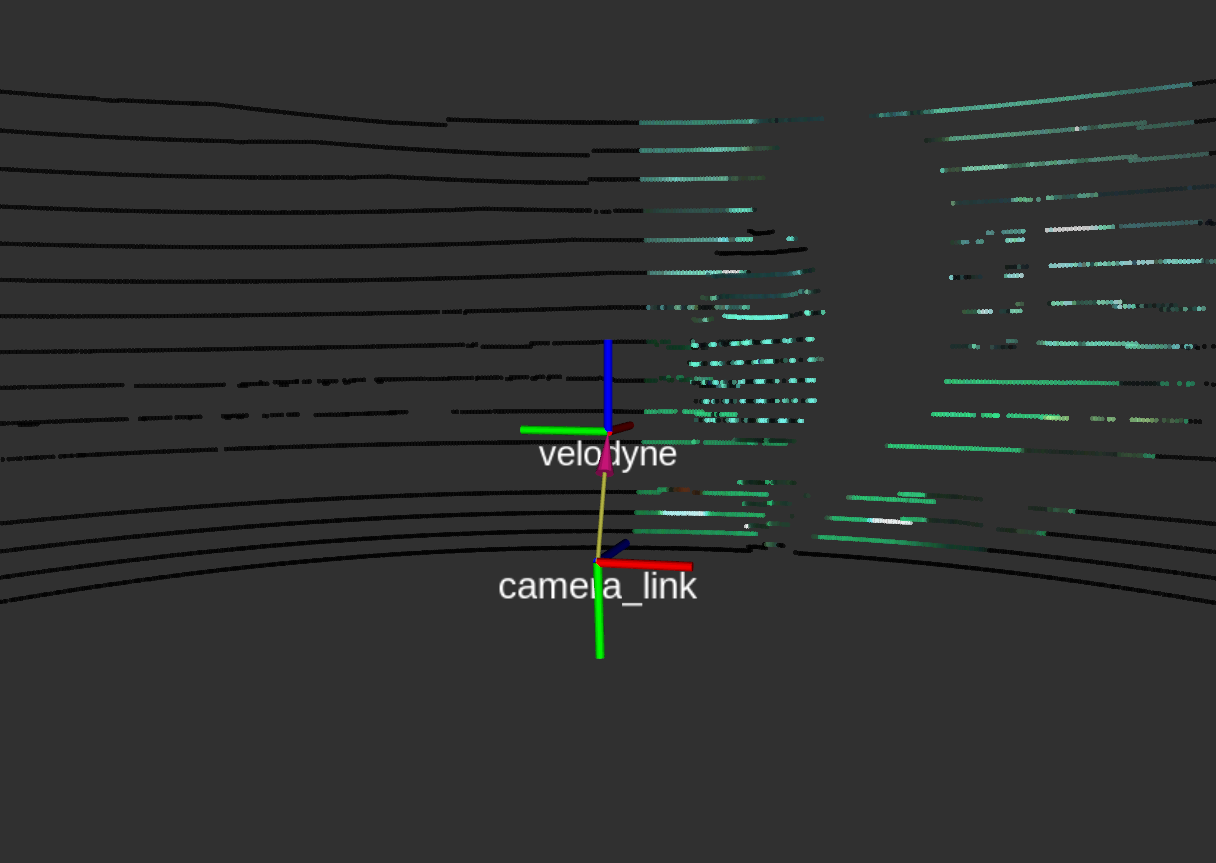
\includegraphics[width=\textwidth]{img/sensor_fusion/cambada_fusion_points.png}
		\caption{The coordinate frames of the \ac{lidar} and the camera are also present on the image. The colored point cloud is represented with points of 4 pixels and 70\% of transparency.}
		\label{fig:sensor-fusion:cambada-points}
	\end{subfigure}
	\qquad
	\begin{subfigure}[c]{0.45\textwidth}
		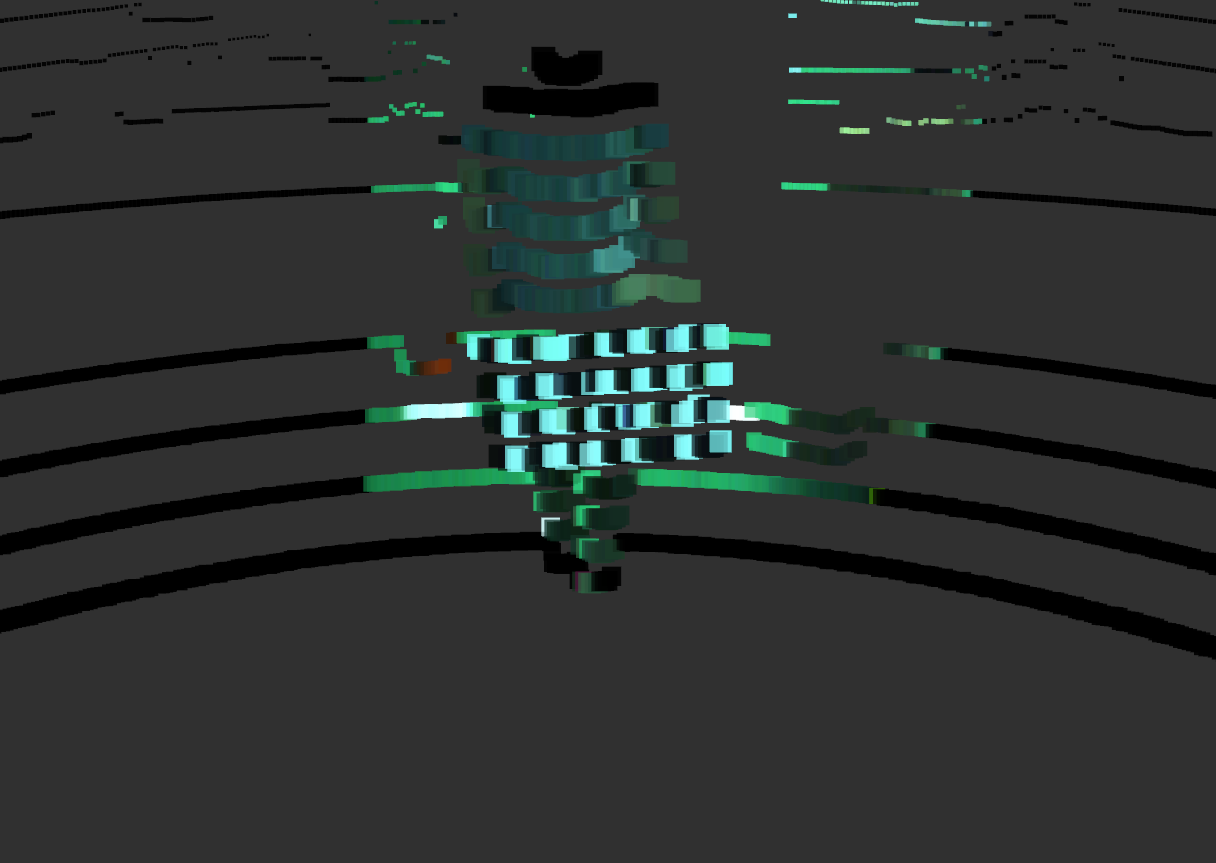
\includegraphics[width=\textwidth]{img/sensor_fusion/cambada_fusion_squares.png}
		\caption{The rectangles presented on the image have a size 4 cm and a transparency of 70\%.}
		\label{fig:sensor-fusion:cambada-squares}
	\end{subfigure}
\caption{Data fusion between the camera and the \ac{lidar} on a \ac{msl} field. The colored point cloud presented with points~\ref{fig:sensor-fusion:cambada-points} or squares~\ref{fig:sensor-fusion:cambada-squares} does not improve significantly the results. Due to the low density of data, it is not immediate the recognition of the ball, box, person and chessboard.}
	\label{fig:cambada-sensor-fusion}
\end{figure}


However, such results are obtained due to a low point density (VLP-16 only has 16 lines of data\footnote{Actually, our Velodyne VLP-16 has one of its lasers broken, therefore we only have 15 lines of data.}) and distance from the objects to the camera (a few meters). Another test, with different objects and on a smaller room, with the objects of interest closer, is shown on figure~\ref{fig:dark-room-sensor-fusion}.

\begin{figure}[H]
	\centering
	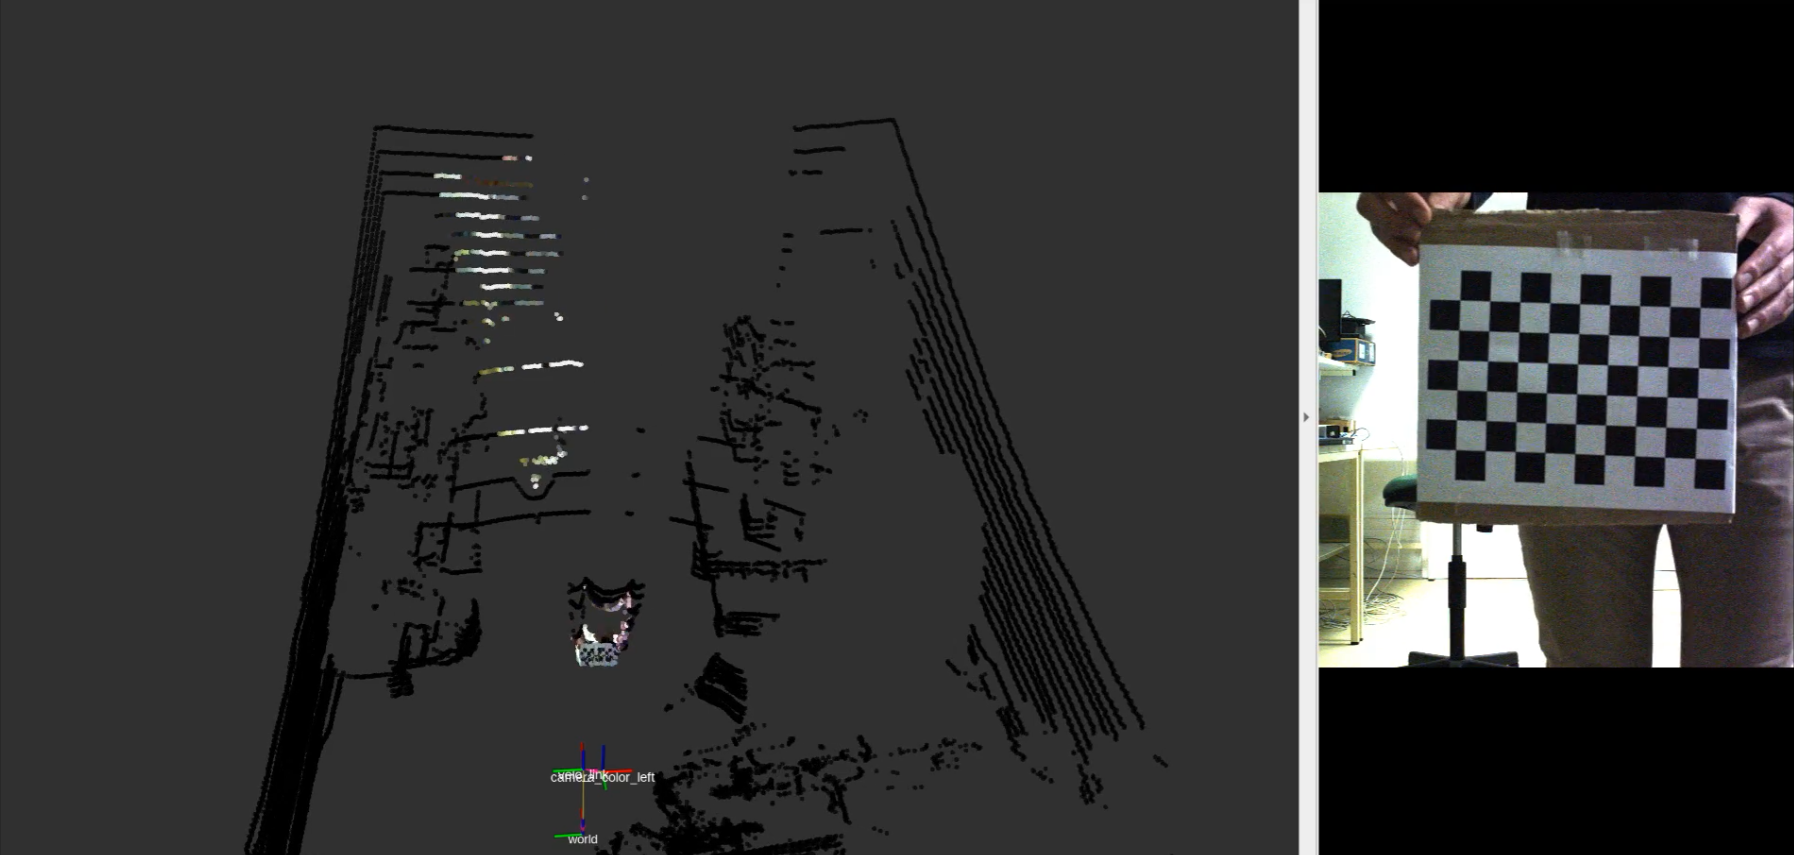
\includegraphics[width=0.7\textwidth]{img/sensor_fusion/dark-room-sensor-fusion.png}
	\caption{Data fusion between the \ac{lidar} and the camera data. On the left is the colored point cloud and on the right the image. The difference between this and the colored point clouds presented on figure~\ref{fig:cambada-sensor-fusion} is that the objects of interest are closer to the camera and the experimental setup is placed inside a small room.}
	\label{fig:dark-room-sensor-fusion}
\end{figure}

Lastly, to demonstrate the effect of point cloud density on point cloud coloring, the nodes developed were applied to \ac{kitti} data set, which uses a Velodyne HDL-64E, with 64 pairs of laser beams and photoreceptors, having $4\times$ more lines than our setup. The resulting colored point cloud is presented on figure~\ref{fig:kitti-sensor-fusion}, and the differences between the figures~\ref{fig:cambada-sensor-fusion} and~\ref{fig:dark-room-sensor-fusion} can clearly be noted from figure~\ref{fig:kitti-sensor-fusion}. 

On figure~\ref{fig:kitti-sensor-fusion} delays between the colored point cloud and the image are visible. That occurs since our implementation cannot run in real time and \ac{kitti} camera data is published at $10 Hz$.

\begin{figure}[H]
	\centering
	\begin{subfigure}[c]{0.45\textwidth}
		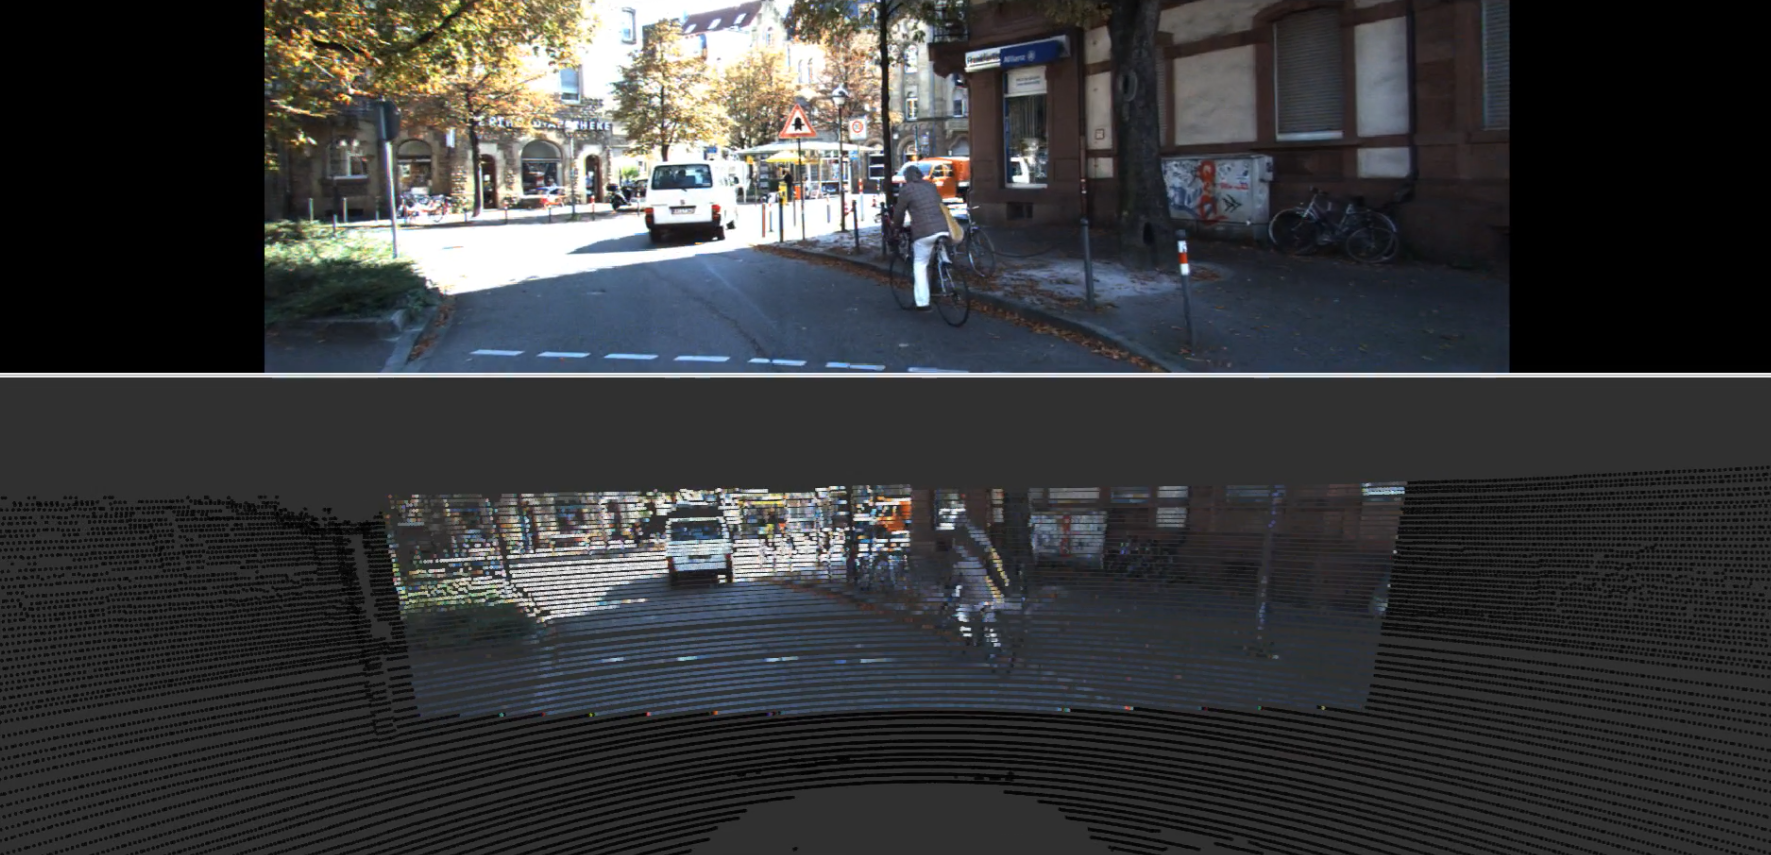
\includegraphics[width=\textwidth]{img/sensor_fusion/kitti-sensor-fusion-1.png}
		\caption{Data fusion on a road scenario from \ac{kitti} dataset. The cyclist and the car can clearly been identified on the colored point cloud. Colored point cloud is represented with Points with 6 pixels of size and 50\% of transparency.}
		\label{fig:kitti-sensor-fusion-1}
	\end{subfigure}
	\qquad
	\begin{subfigure}[c]{0.45\textwidth}
		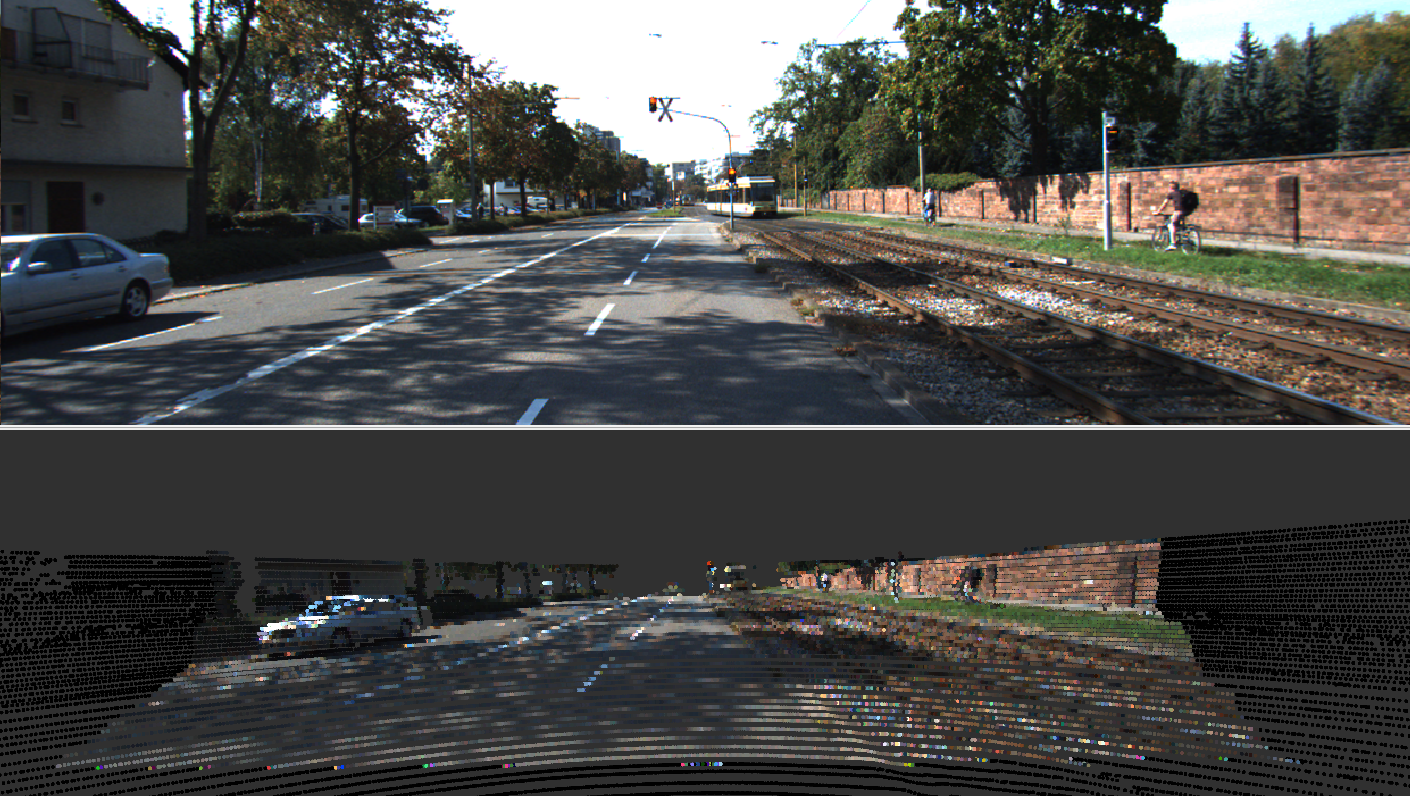
\includegraphics[width=\textwidth]{img/sensor_fusion/kitti-sensor-fusion-2.png}
		\caption{Data fusion on a road scenario from \ac{kitti} dataset. The car, the wall, the road lines and the shadows can clearly be seen on the colored point cloud. Colored point cloud is represented with Points with 6 pixels of size and 50\% of transparency.}
		\label{fig:kitti-sensor-fusion-2}
	\end{subfigure}
	\caption{Data fusion between the camera and the \ac{lidar} on the \ac{kitti} dataset. On the top there is the image and on the bottom the colored point cloud. Note that there is a mismatch between the image being shown and the image used to create the colored point cloud of 2 frames.}
	\label{fig:kitti-sensor-fusion}
\end{figure}


